\documentclass[12pt, twoside]{article}
\usepackage[letterpaper, margin=1in, headsep=0.5in]{geometry}
\usepackage[english]{babel}
\usepackage[utf8]{inputenc}
\usepackage{amsmath}
\usepackage{amsfonts}
\usepackage{amssymb}
\usepackage{tikz}
\usetikzlibrary{quotes, angles}
\usepackage{graphicx}
\usepackage{enumitem}
\usepackage{multicol}

\newif\ifmeta
\metatrue %print standards and topics tags

\title{Regents Geometry}
\author{Chris Huson}
\date{September 2020}

\usepackage{fancyhdr}
\pagestyle{fancy}
\fancyhf{}
\renewcommand{\headrulewidth}{0pt} % disable the underline of the header
\raggedbottom


\fancyhead[LE]{\thepage}
\fancyhead[RO]{\thepage \\ Name: \hspace{4cm} \,\\}
\fancyhead[LO]{BECA / Dr. Huson / Geometry 01-Intro\\* 1.3 Pretest (open book)}

\begin{document}

\subsubsection*{1-3 Classwork: Segment Addition Pretest, Vocabulary}
\begin{enumerate}
\item Do Now: Given $\overline{ABC}$, $AB=2$, and $AC=12$. Find ${BC}$.\\[1cm]
    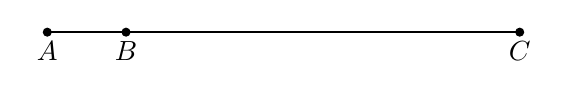
\begin{tikzpicture}
      \draw [-, thick] (1,0)--(7,0);
      \draw [fill] (1,0) circle [radius=0.05] node[below]{$A$};
      \draw [fill] (2,0) circle [radius=0.05] node[below]{$B$};
      \draw [fill] (7,0) circle [radius=0.05] node[below]{$C$};
    \end{tikzpicture} \vspace{2cm}
    
\item Do Now: Given $\overline{DEF}$, $DE=3 \frac{1}{3}$, and $EF=1$.
  \begin{enumerate}
  \item Find ${DF}$.\\[0.75cm]
    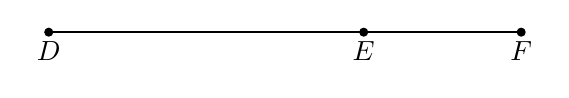
\begin{tikzpicture}
      \draw [-, thick] (1,0)--(7,0);
      \draw [fill] (1,0) circle [radius=0.05] node[below]{$D$};
      \draw [fill] (5,0) circle [radius=0.05] node[below]{$E$};
      \draw [fill] (7,0) circle [radius=0.05] node[below]{$F$};
    \end{tikzpicture} \bigskip
  \item The postulate used in this problem is the \rule{6cm}{0.15mm}.
  \end{enumerate}

\item Do Now: Given $\overline{PQR}$, $PQ=x-2$, $QR=x$, $PR=10$. Find ${PQ}$.
  \begin{enumerate}
  \item Label the diagram with the given values.
  \begin{flushright}
    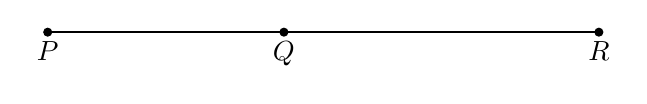
\begin{tikzpicture}
        \draw [-, thick] (0,0)--(7,0);
        \draw [fill] (0,0) circle [radius=0.05] node[below]{$P$};
        \draw [fill] (3,0) circle [radius=0.05] node[below]{$Q$};
        \draw [fill] (7,0) circle [radius=0.05] node[below]{$R$};
    \end{tikzpicture}
  \end{flushright} \vspace{1cm}
  \item Write an equation: \vspace{1cm}
  \item Solve for $x$
  \vspace{3cm}
  \item Answer the question. \\
  Find $PQ$ by substituting for $x$. \vspace{1.5cm}
  \item Check your answer
  \end{enumerate}
  %\vspace{2cm}

\newpage
\item Points that are all located on the same line are $\rule{4cm}{0.15mm}$.

\item Use symbols to write the name of each geometric figure.
  \begin{enumerate}
  \item %Ray DE
    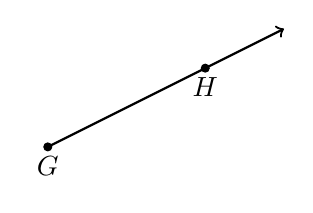
\begin{tikzpicture}
      \draw [->, thick] (0,0)--(3,1.5);
      \draw [fill] (0,0) circle [radius=0.05] node[below]{$G$};
      \draw [fill] (2,1) circle [radius=0.05] node[below]{$H$};
    \end{tikzpicture} \bigskip
  \item \hspace{1cm}%Line AB
    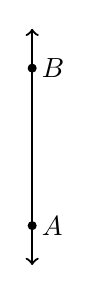
\begin{tikzpicture}
      \draw [<->, thick] (1,0)--(1,3);
      \draw [fill] (1,0.5) circle [radius=0.05] node[right]{$A$};
      \draw [fill] (1,2.5) circle [radius=0.05] node[right]{$B$};
    \end{tikzpicture} \bigskip
    \item %Line segment XY
      \begin{tikzpicture}
        \draw [-, thick] (1,0)--(0,2);
        \draw [fill] (1,0) circle [radius=0.05] node[below]{$E$};
        \draw [fill] (0,2) circle [radius=0.05] node[left]{$F$};
      \end{tikzpicture}
  \end{enumerate}

\item A flat surface is a(n) $\rule{4cm}{0.15mm}$.\bigskip

\item Two line segments or angles of equal measure are $\rule{4cm}{0.15mm}$.\bigskip

\item Identify two rays in the given plane.\\[0.25in]
  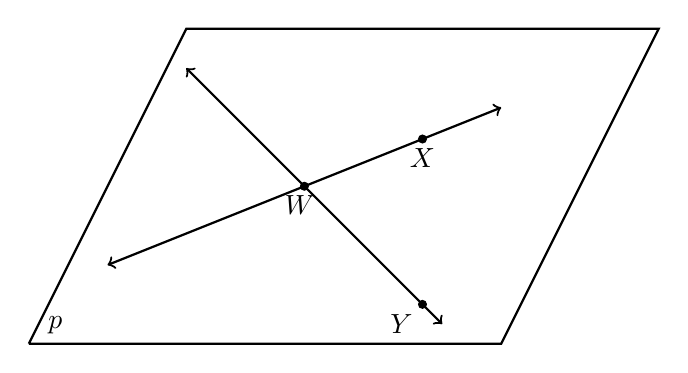
\begin{tikzpicture}
    \draw [thick](0,0) node[above right]{$\ p$} --(6,0)--(8,4)--(2,4)--(0,0);
    \draw [<->, thick] (1,1)--(6,3);
    \draw [fill] (3.5,2) circle [radius=0.05] node[below]{$W \ $};
    \draw [fill] (5,2.6) circle [radius=0.05] node[below]{$X$};
    \draw [<->, thick] (2,3.5)--(5.25,.25);
    \draw [fill] (5,0.5) circle [radius=0.05] node[below left]{$Y$};
  \end{tikzpicture} %\vspace{2cm}

\item Use symbols to write the name of the given figure.
  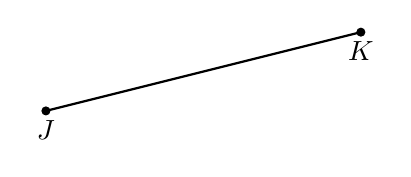
\begin{tikzpicture}
    \draw [-, thick] (0,0)--(4,1);
    \draw [fill] (0,0) circle [radius=0.05] node[below]{$J$};
    \draw [fill] (4,1) circle [radius=0.05] node[below]{$K$};
  \end{tikzpicture} \bigskip

\item A(n) $\rule{4cm}{0.15mm}$ is a portion of a line that includes two points and all of the collinear points between the two points.\smallskip

\newpage
\item Given $\triangle JKL$ with $\overline{JK} \cong \overline{KL}$. On the diagram mark the congruent line segments with tick marks.
  \begin{center}
  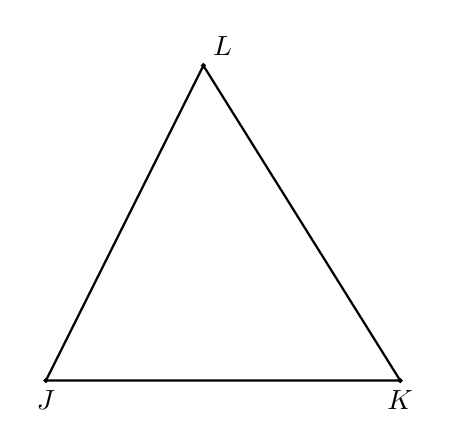
\begin{tikzpicture}[scale=0.5]
    \draw [thick](0,0)--(9,0)--(4,8)--(0,0);
    \draw [fill] (0,0) circle [radius=0.05] node[below]{$J$};
    \draw [fill] (9,0) circle [radius=0.05] node[below]{$K$};
    \draw [fill] (4,8) circle [radius=0.05] node[above right]{$L$};
  \end{tikzpicture}
  \end{center}
  
\item Draw and label a line segment $\overline {AB}$ such that the distance between points $A$ and $B$ is 6 cm. \vspace{2cm}

  
\item Given the rectangle $ABCD$ shown below.
  \begin{enumerate}
    \item Measure and mark the length and width of the rectangle in centimeters.
    \item Calculate the area of the rectangle in square centimeters. (show your work)
  \end{enumerate}
  \vspace{2cm}
  \begin{center}
  \begin{tikzpicture}
    \draw [-, thick] (0,0)--(9,0)--(9,3)--(0,3)--cycle;
    \draw [fill] (0,0) circle [radius=0.05] node[left]{$A$};
    \draw [fill] (9,0) circle [radius=0.05] node[right]{$B$};
    \draw [fill] (9,3) circle [radius=0.05] node[right]{$C$};
    \draw [fill] (0,3) circle [radius=0.05] node[left]{$D$};
  \end{tikzpicture}
  \end{center}

\newpage
\item Early finishers: In the following two problems, solve for the value of $x$.
  \begin{multicols}{2}
    \begin{enumerate}
      \item   $2x+3=x + 9$ \vspace{6cm}
      \item   $\frac{1}{2}(11-x)=5$ \vspace{6cm}
    \end{enumerate}
  \end{multicols}
  \vspace{5cm}

\item Given the linear function $f(x)=3x+4$.
\begin{multicols}{2}
  \begin{enumerate}
    \item Find $f(0)$ \vspace{6cm}
    \item   $f(x)=10$. Find $x$. \vspace{6cm}
  \end{enumerate}
\end{multicols}
  \vspace{6cm}

\item Given $x^2+6x+5=0$. Factor and find the roots. \vspace{4cm}

\end{enumerate}
\end{document}